\begin{frame}
	\frametitle{Gesti\'on}
	
	\begin{itemize}
		\item Se han utilizado metodolog\'ias \'agiles de desarrollo
		\begin{itemize}
			\item Scrum
			\item Kanban
		\end{itemize}
	\end{itemize}
	
\end{frame}

\begin{frame}
	\frametitle{Gesti\'on}
	\framesubtitle{Scrum}
	\begin{columns}[T] % contents are top vertically aligned
		
		\begin{column}[T]{0.5\linewidth} % each column can also be its own 
			\textbf{¿Qu\'e es?}
			\begin{itemize}
				\item M\'etodo de desarrollo iterativo e incremental
				\item En cada ciclo de desarrollo (sprint) se genera un 
				entregable.
				\item Lo importante es que el diferencial de valor incremente
			\end{itemize}
		\end{column}
		\begin{column}[T]{0.5\linewidth} % alternative top-align that's better 
			%for graphics
			\begin{figure}
				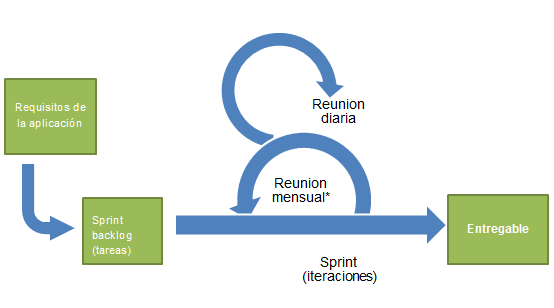
\includegraphics[width=1.0\linewidth]{./Figures/Scrumm.PNG}
				\label{scrum}
			\end{figure}
			\tiny{\url{https://upload.wikimedia.org/wikipedia/commons/e/e5/Scrumm.PNG}
					
					Autor: Maxie Ayala 
					Licenciado bajo 
					\hyperlink{creativecommons.org/licenses/by-sa/3.0/}{CC 
					BY-SA 3.0}}
		\end{column}
	\end{columns}

\end{frame}

\begin{frame}
	\frametitle{Gesti\'on}
	\framesubtitle{Kanban}
	
	\textbf{¿Qu\'e es?}
	\begin{itemize}
		\item blabla
	\end{itemize}
	
\end{frame}